\documentclass[1p]{elsarticle_modified}
%\bibliographystyle{elsarticle-num}

%\usepackage[colorlinks]{hyperref}
%\usepackage{abbrmath_seonhwa} %\Abb, \Ascr, \Acal ,\Abf, \Afrak
\usepackage{amsfonts}
\usepackage{amssymb}
\usepackage{amsmath}
\usepackage{amsthm}
\usepackage{scalefnt}
\usepackage{amsbsy}
\usepackage{kotex}
\usepackage{caption}
\usepackage{subfig}
\usepackage{color}
\usepackage{graphicx}
\usepackage{xcolor} %% white, black, red, green, blue, cyan, magenta, yellow
\usepackage{float}
\usepackage{setspace}
\usepackage{hyperref}

\usepackage{tikz}
\usetikzlibrary{arrows}

\usepackage{multirow}
\usepackage{array} % fixed length table
\usepackage{hhline}

%%%%%%%%%%%%%%%%%%%%%
\makeatletter
\renewcommand*\env@matrix[1][\arraystretch]{%
	\edef\arraystretch{#1}%
	\hskip -\arraycolsep
	\let\@ifnextchar\new@ifnextchar
	\array{*\c@MaxMatrixCols c}}
\makeatother %https://tex.stackexchange.com/questions/14071/how-can-i-increase-the-line-spacing-in-a-matrix
%%%%%%%%%%%%%%%

\usepackage[normalem]{ulem}

\newcommand{\msout}[1]{\ifmmode\text{\sout{\ensuremath{#1}}}\else\sout{#1}\fi}
%SOURCE: \msout is \stkout macro in https://tex.stackexchange.com/questions/20609/strikeout-in-math-mode

\newcommand{\cancel}[1]{
	\ifmmode
	{\color{red}\msout{#1}}
	\else
	{\color{red}\sout{#1}}
	\fi
}

\newcommand{\add}[1]{
	{\color{blue}\uwave{#1}}
}

\newcommand{\replace}[2]{
	\ifmmode
	{\color{red}\msout{#1}}{\color{blue}\uwave{#2}}
	\else
	{\color{red}\sout{#1}}{\color{blue}\uwave{#2}}
	\fi
}

\newcommand{\Sol}{\mathcal{S}} %segment
\newcommand{\D}{D} %diagram
\newcommand{\A}{\mathcal{A}} %arc


%%%%%%%%%%%%%%%%%%%%%%%%%%%%%5 test

\def\sl{\operatorname{\textup{SL}}(2,\Cbb)}
\def\psl{\operatorname{\textup{PSL}}(2,\Cbb)}
\def\quan{\mkern 1mu \triangleright \mkern 1mu}

\theoremstyle{definition}
\newtheorem{thm}{Theorem}[section]
\newtheorem{prop}[thm]{Proposition}
\newtheorem{lem}[thm]{Lemma}
\newtheorem{ques}[thm]{Question}
\newtheorem{cor}[thm]{Corollary}
\newtheorem{defn}[thm]{Definition}
\newtheorem{exam}[thm]{Example}
\newtheorem{rmk}[thm]{Remark}
\newtheorem{alg}[thm]{Algorithm}

\newcommand{\I}{\sqrt{-1}}
\begin{document}

%\begin{frontmatter}
%
%\title{Boundary parabolic representations of knots up to 8 crossings}
%
%%% Group authors per affiliation:
%\author{Yunhi Cho} 
%\address{Department of Mathematics, University of Seoul, Seoul, Korea}
%\ead{yhcho@uos.ac.kr}
%
%
%\author{Seonhwa Kim} %\fnref{s_kim}}
%\address{Center for Geometry and Physics, Institute for Basic Science, Pohang, 37673, Korea}
%\ead{ryeona17@ibs.re.kr}
%
%\author{Hyuk Kim}
%\address{Department of Mathematical Sciences, Seoul National University, Seoul 08826, Korea}
%\ead{hyukkim@snu.ac.kr}
%
%\author{Seokbeom Yoon}
%\address{Department of Mathematical Sciences, Seoul National University, Seoul, 08826,  Korea}
%\ead{sbyoon15@snu.ac.kr}
%
%\begin{abstract}
%We find all boundary parabolic representation of knots up to 8 crossings.
%
%\end{abstract}
%\begin{keyword}
%    \MSC[2010] 57M25 
%\end{keyword}
%
%\end{frontmatter}

%\linenumbers
%\tableofcontents
%
\newcommand\colored[1]{\textcolor{white}{\rule[-0.35ex]{0.8em}{1.4ex}}\kern-0.8em\color{red} #1}%
%\newcommand\colored[1]{\textcolor{white}{ #1}\kern-2.17ex	\textcolor{white}{ #1}\kern-1.81ex	\textcolor{white}{ #1}\kern-2.15ex\color{red}#1	}

{\Large $\underline{12n_{0371}~(K12n_{0371})}$}

\setlength{\tabcolsep}{10pt}
\renewcommand{\arraystretch}{1.6}
\vspace{1cm}\begin{tabular}{m{100pt}>{\centering\arraybackslash}m{274pt}}
\multirow{5}{120pt}{
	\centering
	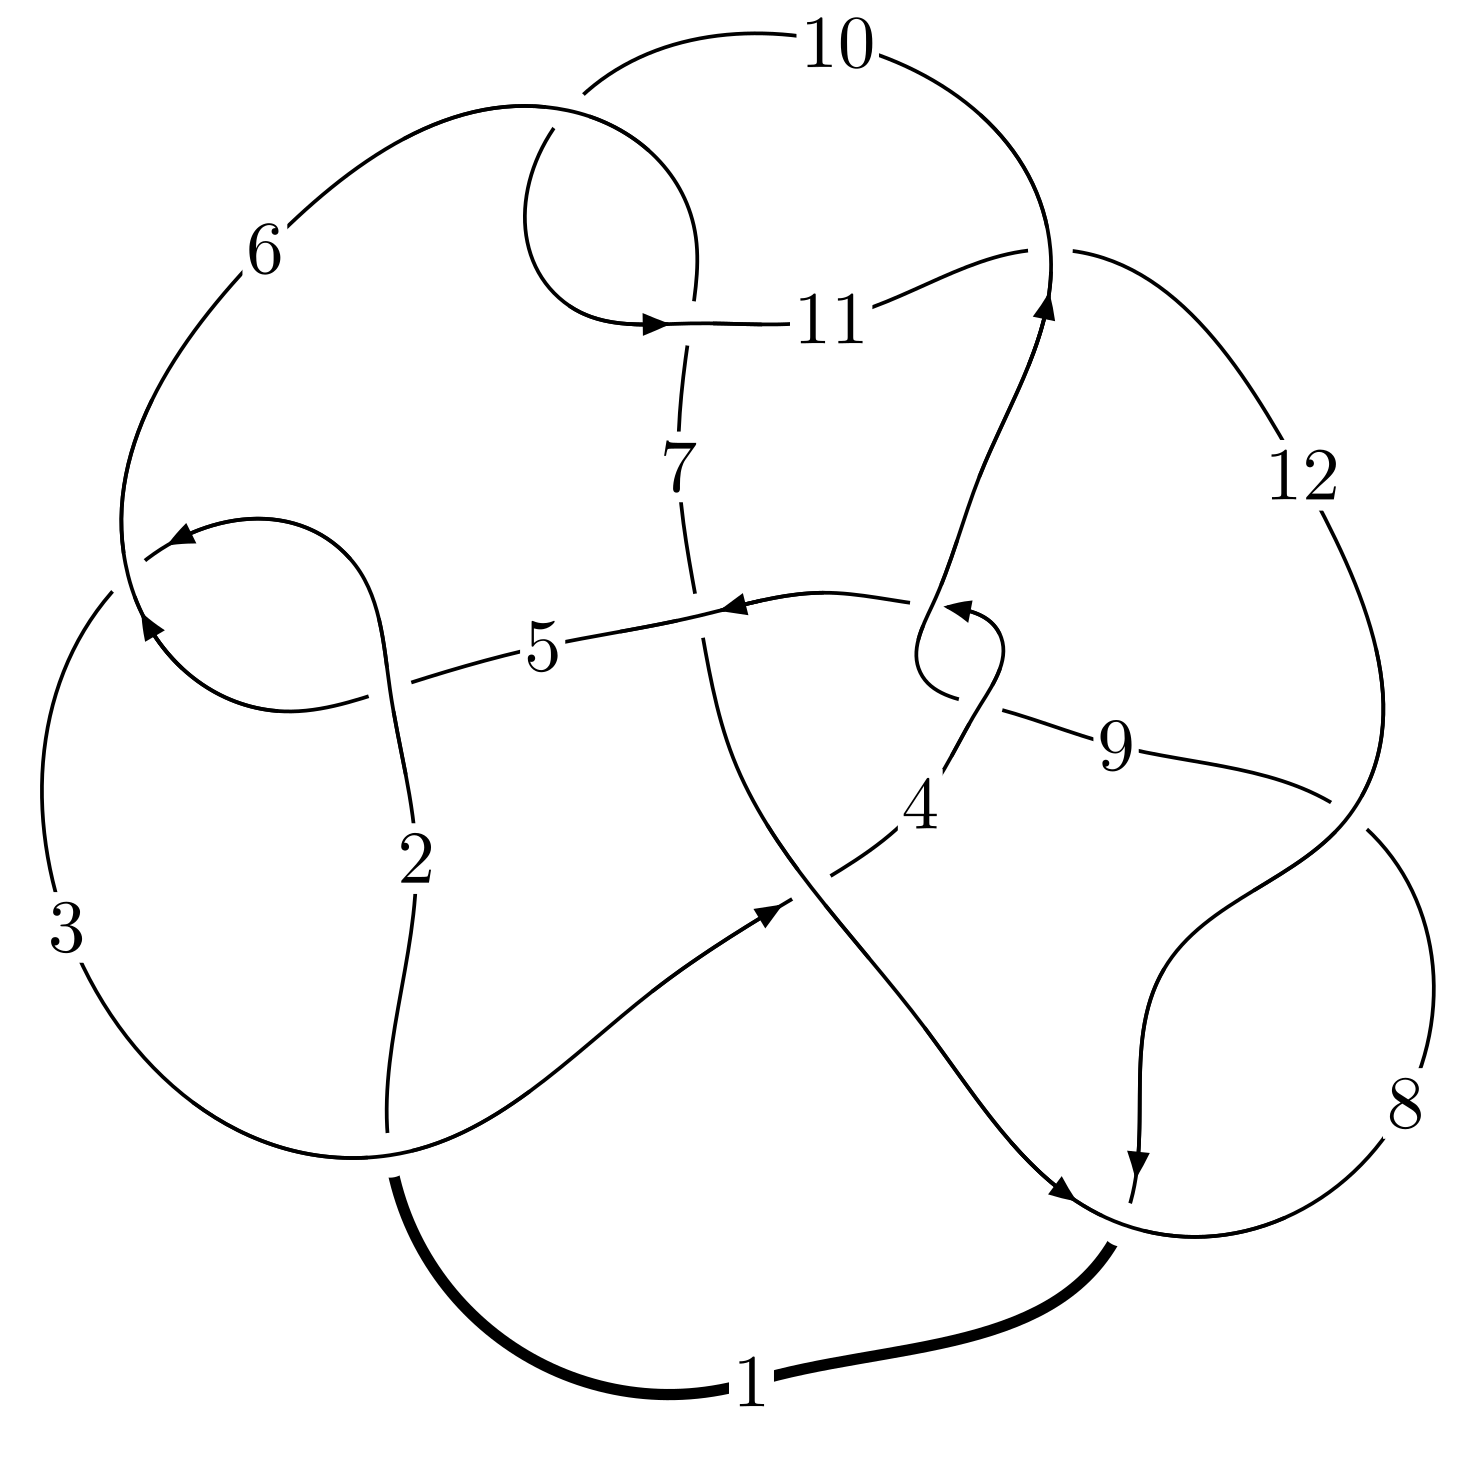
\includegraphics[width=112pt]{../../../GIT/diagram.site/Diagrams/png/2460_12n_0371.png}\\
\ \ \ A knot diagram\footnotemark}&
\allowdisplaybreaks
\textbf{Linearized knot diagam} \\
\cline{2-2}
 &
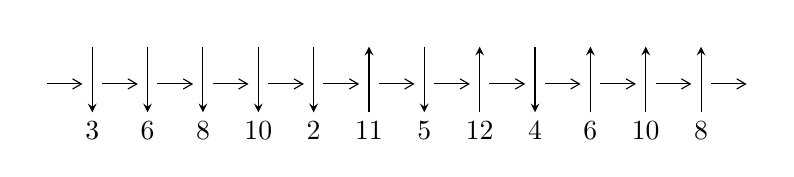
\begin{tikzpicture}[x=20pt, y=17pt]
	% nodes
	\node (C0) at (0, 0) {};
	\node (C1) at (1, 0) {};
	\node (C1U) at (1, +1) {};
	\node (C1D) at (1, -1) {3};

	\node (C2) at (2, 0) {};
	\node (C2U) at (2, +1) {};
	\node (C2D) at (2, -1) {6};

	\node (C3) at (3, 0) {};
	\node (C3U) at (3, +1) {};
	\node (C3D) at (3, -1) {8};

	\node (C4) at (4, 0) {};
	\node (C4U) at (4, +1) {};
	\node (C4D) at (4, -1) {10};

	\node (C5) at (5, 0) {};
	\node (C5U) at (5, +1) {};
	\node (C5D) at (5, -1) {2};

	\node (C6) at (6, 0) {};
	\node (C6U) at (6, +1) {};
	\node (C6D) at (6, -1) {11};

	\node (C7) at (7, 0) {};
	\node (C7U) at (7, +1) {};
	\node (C7D) at (7, -1) {5};

	\node (C8) at (8, 0) {};
	\node (C8U) at (8, +1) {};
	\node (C8D) at (8, -1) {12};

	\node (C9) at (9, 0) {};
	\node (C9U) at (9, +1) {};
	\node (C9D) at (9, -1) {4};

	\node (C10) at (10, 0) {};
	\node (C10U) at (10, +1) {};
	\node (C10D) at (10, -1) {6};

	\node (C11) at (11, 0) {};
	\node (C11U) at (11, +1) {};
	\node (C11D) at (11, -1) {10};

	\node (C12) at (12, 0) {};
	\node (C12U) at (12, +1) {};
	\node (C12D) at (12, -1) {8};
	\node (C13) at (13, 0) {};

	% arrows
	\draw[->,>={angle 60}]
	(C0) edge (C1) (C1) edge (C2) (C2) edge (C3) (C3) edge (C4) (C4) edge (C5) (C5) edge (C6) (C6) edge (C7) (C7) edge (C8) (C8) edge (C9) (C9) edge (C10) (C10) edge (C11) (C11) edge (C12) (C12) edge (C13) ;	\draw[->,>=stealth]
	(C1U) edge (C1D) (C2U) edge (C2D) (C3U) edge (C3D) (C4U) edge (C4D) (C5U) edge (C5D) (C6D) edge (C6U) (C7U) edge (C7D) (C8D) edge (C8U) (C9U) edge (C9D) (C10D) edge (C10U) (C11D) edge (C11U) (C12D) edge (C12U) ;
	\end{tikzpicture} \\
\hhline{~~} \\& 
\textbf{Solving Sequence} \\ \cline{2-2} 
 &
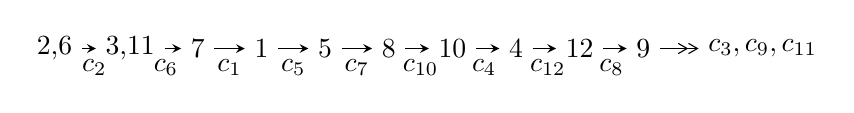
\begin{tikzpicture}[x=23pt, y=7pt]
	% node
	\node (A0) at (-1/8, 0) {2,6};
	\node (A1) at (17/16, 0) {3,11};
	\node (A2) at (17/8, 0) {7};
	\node (A3) at (25/8, 0) {1};
	\node (A4) at (33/8, 0) {5};
	\node (A5) at (41/8, 0) {8};
	\node (A6) at (49/8, 0) {10};
	\node (A7) at (57/8, 0) {4};
	\node (A8) at (65/8, 0) {12};
	\node (A9) at (73/8, 0) {9};
	\node (C1) at (1/2, -1) {$c_{2}$};
	\node (C2) at (13/8, -1) {$c_{6}$};
	\node (C3) at (21/8, -1) {$c_{1}$};
	\node (C4) at (29/8, -1) {$c_{5}$};
	\node (C5) at (37/8, -1) {$c_{7}$};
	\node (C6) at (45/8, -1) {$c_{10}$};
	\node (C7) at (53/8, -1) {$c_{4}$};
	\node (C8) at (61/8, -1) {$c_{12}$};
	\node (C9) at (69/8, -1) {$c_{8}$};
	\node (A10) at (11, 0) {$c_{3},c_{9},c_{11}$};

	% edge
	\draw[->,>=stealth]	
	(A0) edge (A1) (A1) edge (A2) (A2) edge (A3) (A3) edge (A4) (A4) edge (A5) (A5) edge (A6) (A6) edge (A7) (A7) edge (A8) (A8) edge (A9) ;
	\draw[->>,>={angle 60}]	
	(A9) edge (A10);
\end{tikzpicture} \\ 

\end{tabular} \\

\footnotetext{
The image of knot diagram is generated by the software ``\textbf{Draw programme}" developed by Andrew Bartholomew(\url{http://www.layer8.co.uk/maths/draw/index.htm\#Running-draw}), where we modified some parts for our purpose(\url{https://github.com/CATsTAILs/LinksPainter}).
}\phantom \\ \newline 
\centering \textbf{Ideals for irreducible components\footnotemark of $X_{\text{par}}$} 
 
\begin{align*}
I^u_{1}&=\langle 
2 u^{13}-7 u^{12}+11 u^{11}-7 u^{10}+10 u^9-33 u^8+54 u^7-34 u^6+u^5+5 u^4+u^3+4 u^2+b-5 u+1,\\
\phantom{I^u_{1}}&\phantom{= \langle  }2 u^{13}-7 u^{12}+11 u^{11}-7 u^{10}+10 u^9-33 u^8+54 u^7-34 u^6+u^5+5 u^4+u^3+4 u^2+a-6 u+1,\\
\phantom{I^u_{1}}&\phantom{= \langle  }u^{15}-4 u^{14}+7 u^{13}-5 u^{12}+4 u^{11}-16 u^{10}+33 u^9-25 u^8-4 u^7+17 u^6-6 u^5- u^4-2 u^3+2 u^2+u-1\rangle \\
I^u_{2}&=\langle 
u^9+3 u^8+4 u^7-4 u^5-4 u^4+b+u,\;u^9+3 u^8+4 u^7-4 u^5-4 u^4+a,\;u^{10}+3 u^9+4 u^8-4 u^6-4 u^5+u^3+u^2-1\rangle \\
\\
\end{align*}
\raggedright * 2 irreducible components of $\dim_{\mathbb{C}}=0$, with total 25 representations.\\
\footnotetext{All coefficients of polynomials are rational numbers. But the coefficients are sometimes approximated in decimal forms when there is not enough margin.}
\newpage
\renewcommand{\arraystretch}{1}
\centering \section*{I. $I^u_{1}= \langle 2 u^{13}-7 u^{12}+\cdots+b+1,\;2 u^{13}-7 u^{12}+\cdots+a+1,\;u^{15}-4 u^{14}+\cdots+u-1 \rangle$}
\flushleft \textbf{(i) Arc colorings}\\
\begin{tabular}{m{7pt} m{180pt} m{7pt} m{180pt} }
\flushright $a_{2}=$&$\begin{pmatrix}1\\0\end{pmatrix}$ \\
\flushright $a_{6}=$&$\begin{pmatrix}0\\u\end{pmatrix}$ \\
\flushright $a_{3}=$&$\begin{pmatrix}1\\u^2\end{pmatrix}$ \\
\flushright $a_{11}=$&$\begin{pmatrix}-2 u^{13}+7 u^{12}+\cdots+6 u-1\\-2 u^{13}+7 u^{12}+\cdots+5 u-1\end{pmatrix}$ \\
\flushright $a_{7}=$&$\begin{pmatrix}-3 u^{13}+11 u^{12}+\cdots+7 u-2\\u^{14}-6 u^{13}+\cdots-6 u^2+6 u\end{pmatrix}$ \\
\flushright $a_{1}=$&$\begin{pmatrix}- u^2+1\\- u^4\end{pmatrix}$ \\
\flushright $a_{5}=$&$\begin{pmatrix}u\\u\end{pmatrix}$ \\
\flushright $a_{8}=$&$\begin{pmatrix}-3 u^{13}+11 u^{12}+\cdots+7 u-3\\u^{14}-6 u^{13}+\cdots+6 u-1\end{pmatrix}$ \\
\flushright $a_{10}=$&$\begin{pmatrix}-2 u^{13}+7 u^{12}+\cdots+6 u-1\\- u^{14}+u^{13}+\cdots+7 u-3\end{pmatrix}$ \\
\flushright $a_{4}=$&$\begin{pmatrix}u^{11}-2 u^{10}+u^9+5 u^7-10 u^6+5 u^5+u^3- u^2+1\\u^{13}-2 u^{12}+2 u^{11}- u^{10}+5 u^9-10 u^8+10 u^7-5 u^6+u^5- u^4+u^3+u^2\end{pmatrix}$ \\
\flushright $a_{12}=$&$\begin{pmatrix}- u^{12}+3 u^{11}+\cdots-2 u^2+1\\- u^{14}+3 u^{13}+\cdots-3 u^4+u^3\end{pmatrix}$ \\
\flushright $a_{9}=$&$\begin{pmatrix}u^{13}-5 u^{12}+\cdots-6 u+3\\u^{14}-2 u^{13}+\cdots-7 u+5\end{pmatrix}$\\&\end{tabular}
\flushleft \textbf{(ii) Obstruction class $= -1$}\\~\\
\flushleft \textbf{(iii) Cusp Shapes $= 4 u^{13}-14 u^{12}+19 u^{11}-7 u^{10}+13 u^9-68 u^8+98 u^7-35 u^6-33 u^5+23 u^3+3 u^2-14 u-6$}\\~\\
\newpage\renewcommand{\arraystretch}{1}
\flushleft \textbf{(iv) u-Polynomials at the component}\newline \\
\begin{tabular}{m{50pt}|m{274pt}}
Crossings & \hspace{64pt}u-Polynomials at each crossing \\
\hline $$\begin{aligned}c_{1}\end{aligned}$$&$\begin{aligned}
&u^{15}+2 u^{14}+\cdots+5 u+1
\end{aligned}$\\
\hline $$\begin{aligned}c_{2},c_{5}\end{aligned}$$&$\begin{aligned}
&u^{15}+4 u^{14}+\cdots+u+1
\end{aligned}$\\
\hline $$\begin{aligned}c_{3}\end{aligned}$$&$\begin{aligned}
&u^{15}-10 u^{13}+\cdots+4 u+1
\end{aligned}$\\
\hline $$\begin{aligned}c_{4},c_{7},c_{9}\end{aligned}$$&$\begin{aligned}
&u^{15}- u^{14}+\cdots+2 u+1
\end{aligned}$\\
\hline $$\begin{aligned}c_{6},c_{10}\end{aligned}$$&$\begin{aligned}
&u^{15}+14 u^{14}+\cdots+240 u+32
\end{aligned}$\\
\hline $$\begin{aligned}c_{8},c_{12}\end{aligned}$$&$\begin{aligned}
&u^{15}+4 u^{14}+\cdots+9 u+1
\end{aligned}$\\
\hline $$\begin{aligned}c_{11}\end{aligned}$$&$\begin{aligned}
&u^{15}-10 u^{14}+\cdots+12032 u-1024
\end{aligned}$\\
\hline
\end{tabular}\\~\\
\newpage\renewcommand{\arraystretch}{1}
\flushleft \textbf{(v) Riley Polynomials at the component}\newline \\
\begin{tabular}{m{50pt}|m{274pt}}
Crossings & \hspace{64pt}Riley Polynomials at each crossing \\
\hline $$\begin{aligned}c_{1}\end{aligned}$$&$\begin{aligned}
&y^{15}+30 y^{14}+\cdots+5 y-1
\end{aligned}$\\
\hline $$\begin{aligned}c_{2},c_{5}\end{aligned}$$&$\begin{aligned}
&y^{15}-2 y^{14}+\cdots+5 y-1
\end{aligned}$\\
\hline $$\begin{aligned}c_{3}\end{aligned}$$&$\begin{aligned}
&y^{15}-20 y^{14}+\cdots-2 y-1
\end{aligned}$\\
\hline $$\begin{aligned}c_{4},c_{7},c_{9}\end{aligned}$$&$\begin{aligned}
&y^{15}-35 y^{14}+\cdots-6 y-1
\end{aligned}$\\
\hline $$\begin{aligned}c_{6},c_{10}\end{aligned}$$&$\begin{aligned}
&y^{15}-10 y^{14}+\cdots+12032 y-1024
\end{aligned}$\\
\hline $$\begin{aligned}c_{8},c_{12}\end{aligned}$$&$\begin{aligned}
&y^{15}+24 y^{14}+\cdots+89 y-1
\end{aligned}$\\
\hline $$\begin{aligned}c_{11}\end{aligned}$$&$\begin{aligned}
&y^{15}+78 y^{14}+\cdots+66256896 y-1048576
\end{aligned}$\\
\hline
\end{tabular}\\~\\
\newpage\flushleft \textbf{(vi) Complex Volumes and Cusp Shapes}
$$\begin{array}{c|c|c}  
\text{Solutions to }I^u_{1}& \I (\text{vol} + \sqrt{-1}CS) & \text{Cusp shape}\\
 \hline 
\begin{aligned}
u &= \phantom{-}0.712549 + 0.633880 I \\
a &= \phantom{-}0.274451 - 1.191860 I \\
b &= -0.43810 - 1.82574 I\end{aligned}
 & -1.05212 - 4.72304 I & -2.71866 + 7.35913 I \\ \hline\begin{aligned}
u &= \phantom{-}0.712549 - 0.633880 I \\
a &= \phantom{-}0.274451 + 1.191860 I \\
b &= -0.43810 + 1.82574 I\end{aligned}
 & -1.05212 + 4.72304 I & -2.71866 - 7.35913 I \\ \hline\begin{aligned}
u &= \phantom{-}0.815797 + 0.485623 I \\
a &= \phantom{-}1.042200 + 0.113566 I \\
b &= \phantom{-}0.226400 - 0.372057 I\end{aligned}
 & -1.57751 + 0.34385 I & -3.36524 - 0.94481 I \\ \hline\begin{aligned}
u &= \phantom{-}0.815797 - 0.485623 I \\
a &= \phantom{-}1.042200 - 0.113566 I \\
b &= \phantom{-}0.226400 + 0.372057 I\end{aligned}
 & -1.57751 - 0.34385 I & -3.36524 + 0.94481 I \\ \hline\begin{aligned}
u &= \phantom{-}0.766118\phantom{ +0.000000I} \\
a &= \phantom{-}0.453886\phantom{ +0.000000I} \\
b &= -0.312232\phantom{ +0.000000I}\end{aligned}
 & -1.00577\phantom{ +0.000000I} & -12.0370\phantom{ +0.000000I} \\ \hline\begin{aligned}
u &= -0.635896 + 0.026087 I \\
a &= -1.32826 - 1.25555 I \\
b &= -0.69236 - 1.28163 I\end{aligned}
 & -3.88717 + 2.88458 I & -6.82119 + 2.09374 I \\ \hline\begin{aligned}
u &= -0.635896 - 0.026087 I \\
a &= -1.32826 + 1.25555 I \\
b &= -0.69236 + 1.28163 I\end{aligned}
 & -3.88717 - 2.88458 I & -6.82119 - 2.09374 I \\ \hline\begin{aligned}
u &= -0.289639 + 0.547664 I \\
a &= -0.006426 + 1.347820 I \\
b &= \phantom{-}0.283213 + 0.800152 I\end{aligned}
 & \phantom{-}1.30871 + 0.90771 I & \phantom{-}3.11296 - 2.32958 I \\ \hline\begin{aligned}
u &= -0.289639 - 0.547664 I \\
a &= -0.006426 - 1.347820 I \\
b &= \phantom{-}0.283213 - 0.800152 I\end{aligned}
 & \phantom{-}1.30871 - 0.90771 I & \phantom{-}3.11296 + 2.32958 I \\ \hline\begin{aligned}
u &= \phantom{-}1.07267 + 0.99560 I \\
a &= \phantom{-}0.05227 - 1.45647 I \\
b &= -1.02040 - 2.45206 I\end{aligned}
 & -11.1785 - 9.6087 I & -3.50462 + 4.00725 I\\
 \hline 
 \end{array}$$\newpage$$\begin{array}{c|c|c}  
\text{Solutions to }I^u_{1}& \I (\text{vol} + \sqrt{-1}CS) & \text{Cusp shape}\\
 \hline 
\begin{aligned}
u &= \phantom{-}1.07267 - 0.99560 I \\
a &= \phantom{-}0.05227 + 1.45647 I \\
b &= -1.02040 + 2.45206 I\end{aligned}
 & -11.1785 + 9.6087 I & -3.50462 - 4.00725 I \\ \hline\begin{aligned}
u &= \phantom{-}0.99469 + 1.08421 I \\
a &= \phantom{-}1.49910 - 0.14023 I \\
b &= \phantom{-}0.504408 - 1.224440 I\end{aligned}
 & -10.84830 + 1.98719 I & -3.37763 - 0.18602 I \\ \hline\begin{aligned}
u &= \phantom{-}0.99469 - 1.08421 I \\
a &= \phantom{-}1.49910 + 0.14023 I \\
b &= \phantom{-}0.504408 + 1.224440 I\end{aligned}
 & -10.84830 - 1.98719 I & -3.37763 + 0.18602 I \\ \hline\begin{aligned}
u &= -1.05323 + 1.04849 I \\
a &= -0.760279 - 0.943123 I \\
b &= \phantom{-}0.29295 - 1.99161 I\end{aligned}
 & \phantom{-}10.46600 + 3.87226 I & -4.30716 - 1.63349 I \\ \hline\begin{aligned}
u &= -1.05323 - 1.04849 I \\
a &= -0.760279 + 0.943123 I \\
b &= \phantom{-}0.29295 + 1.99161 I\end{aligned}
 & \phantom{-}10.46600 - 3.87226 I & -4.30716 + 1.63349 I\\
 \hline 
 \end{array}$$\newpage\newpage\renewcommand{\arraystretch}{1}
\centering \section*{II. $I^u_{2}= \langle u^9+3 u^8+4 u^7-4 u^5-4 u^4+b+u,\;u^9+3 u^8+4 u^7-4 u^5-4 u^4+a,\;u^{10}+3 u^9+4 u^8-4 u^6-4 u^5+u^3+u^2-1 \rangle$}
\flushleft \textbf{(i) Arc colorings}\\
\begin{tabular}{m{7pt} m{180pt} m{7pt} m{180pt} }
\flushright $a_{2}=$&$\begin{pmatrix}1\\0\end{pmatrix}$ \\
\flushright $a_{6}=$&$\begin{pmatrix}0\\u\end{pmatrix}$ \\
\flushright $a_{3}=$&$\begin{pmatrix}1\\u^2\end{pmatrix}$ \\
\flushright $a_{11}=$&$\begin{pmatrix}- u^9-3 u^8-4 u^7+4 u^5+4 u^4\\- u^9-3 u^8-4 u^7+4 u^5+4 u^4- u\end{pmatrix}$ \\
\flushright $a_{7}=$&$\begin{pmatrix}u^9+3 u^8+4 u^7-3 u^5-2 u^4+u^3- u^2- u\\u^9+3 u^8+4 u^7-3 u^5-3 u^4- u^2+u\end{pmatrix}$ \\
\flushright $a_{1}=$&$\begin{pmatrix}- u^2+1\\- u^4\end{pmatrix}$ \\
\flushright $a_{5}=$&$\begin{pmatrix}u\\u\end{pmatrix}$ \\
\flushright $a_{8}=$&$\begin{pmatrix}u^9+3 u^8+4 u^7+u^6-2 u^5-2 u^4- u^3- u^2- u\\u^9+3 u^8+4 u^7+u^6-2 u^5-3 u^4-2 u^3- u^2+u\end{pmatrix}$ \\
\flushright $a_{10}=$&$\begin{pmatrix}- u^9-3 u^8-4 u^7+4 u^5+4 u^4\\- u^9-3 u^8-4 u^7+4 u^5+5 u^4+u^3-2 u\end{pmatrix}$ \\
\flushright $a_{4}=$&$\begin{pmatrix}- u^7-2 u^6- u^5+3 u^4+3 u^3- u\\- u^9-2 u^8-2 u^7+2 u^6+3 u^5+3 u^4- u^3- u\end{pmatrix}$ \\
\flushright $a_{12}=$&$\begin{pmatrix}- u^8-3 u^7-3 u^6+2 u^5+6 u^4+3 u^3-2 u^2-2 u\\u^6+2 u^5+u^4- u^3- u^2- u-1\end{pmatrix}$ \\
\flushright $a_{9}=$&$\begin{pmatrix}- u^8-3 u^7-3 u^6+2 u^5+5 u^4+u^3-2 u^2+1\\- u^8-2 u^7-2 u^6+u^5+2 u^4+2 u^3+u^2-1\end{pmatrix}$\\&\end{tabular}
\flushleft \textbf{(ii) Obstruction class $= 1$}\\~\\
\flushleft \textbf{(iii) Cusp Shapes $= u^9-6 u^7-13 u^6-3 u^5+11 u^4+16 u^3+5 u^2+u-8$}\\~\\
\newpage\renewcommand{\arraystretch}{1}
\flushleft \textbf{(iv) u-Polynomials at the component}\newline \\
\begin{tabular}{m{50pt}|m{274pt}}
Crossings & \hspace{64pt}u-Polynomials at each crossing \\
\hline $$\begin{aligned}c_{1}\end{aligned}$$&$\begin{aligned}
&u^{10}- u^9+8 u^8-8 u^7+12 u^6-10 u^5-8 u^4+7 u^3+u^2-2 u+1
\end{aligned}$\\
\hline $$\begin{aligned}c_{2}\end{aligned}$$&$\begin{aligned}
&u^{10}+3 u^9+4 u^8-4 u^6-4 u^5+u^3+u^2-1
\end{aligned}$\\
\hline $$\begin{aligned}c_{3}\end{aligned}$$&$\begin{aligned}
&u^{10}- u^9+3 u^8-5 u^6+5 u^5-11 u^4+10 u^3-5 u^2+5 u-1
\end{aligned}$\\
\hline $$\begin{aligned}c_{4},c_{7}\end{aligned}$$&$\begin{aligned}
&u^{10}+u^8+3 u^7+5 u^5+10 u^4+13 u^3+11 u^2+7 u+1
\end{aligned}$\\
\hline $$\begin{aligned}c_{5}\end{aligned}$$&$\begin{aligned}
&u^{10}-3 u^9+4 u^8-4 u^6+4 u^5- u^3+u^2-1
\end{aligned}$\\
\hline $$\begin{aligned}c_{6}\end{aligned}$$&$\begin{aligned}
&u^{10}-5 u^8+3 u^7+10 u^6-8 u^5-6 u^4+8 u^3+2 u^2-3 u-1
\end{aligned}$\\
\hline $$\begin{aligned}c_{8}\end{aligned}$$&$\begin{aligned}
&u^{10}+3 u^9+3 u^8+u^7-4 u^6-9 u^5-6 u^4+3 u^3+11 u^2+2 u-1
\end{aligned}$\\
\hline $$\begin{aligned}c_{9}\end{aligned}$$&$\begin{aligned}
&u^{10}+u^8-3 u^7-5 u^5+10 u^4-13 u^3+11 u^2-7 u+1
\end{aligned}$\\
\hline $$\begin{aligned}c_{10}\end{aligned}$$&$\begin{aligned}
&u^{10}-5 u^8-3 u^7+10 u^6+8 u^5-6 u^4-8 u^3+2 u^2+3 u-1
\end{aligned}$\\
\hline $$\begin{aligned}c_{11}\end{aligned}$$&$\begin{aligned}
&u^{10}-10 u^9+\cdots-13 u+1
\end{aligned}$\\
\hline $$\begin{aligned}c_{12}\end{aligned}$$&$\begin{aligned}
&u^{10}-3 u^9+3 u^8- u^7-4 u^6+9 u^5-6 u^4-3 u^3+11 u^2-2 u-1
\end{aligned}$\\
\hline
\end{tabular}\\~\\
\newpage\renewcommand{\arraystretch}{1}
\flushleft \textbf{(v) Riley Polynomials at the component}\newline \\
\begin{tabular}{m{50pt}|m{274pt}}
Crossings & \hspace{64pt}Riley Polynomials at each crossing \\
\hline $$\begin{aligned}c_{1}\end{aligned}$$&$\begin{aligned}
&y^{10}+15 y^9+\cdots-2 y+1
\end{aligned}$\\
\hline $$\begin{aligned}c_{2},c_{5}\end{aligned}$$&$\begin{aligned}
&y^{10}- y^9+8 y^8-8 y^7+12 y^6-10 y^5-8 y^4+7 y^3+y^2-2 y+1
\end{aligned}$\\
\hline $$\begin{aligned}c_{3}\end{aligned}$$&$\begin{aligned}
&y^{10}+5 y^9- y^8-42 y^7-31 y^6+63 y^5+65 y^4-30 y^3-53 y^2-15 y+1
\end{aligned}$\\
\hline $$\begin{aligned}c_{4},c_{7},c_{9}\end{aligned}$$&$\begin{aligned}
&y^{10}+2 y^9+y^8+11 y^7+12 y^6-79 y^5-70 y^4-19 y^3-41 y^2-27 y+1
\end{aligned}$\\
\hline $$\begin{aligned}c_{6},c_{10}\end{aligned}$$&$\begin{aligned}
&y^{10}-10 y^9+\cdots-13 y+1
\end{aligned}$\\
\hline $$\begin{aligned}c_{8},c_{12}\end{aligned}$$&$\begin{aligned}
&y^{10}-3 y^9-5 y^8+17 y^7+2 y^6+13 y^5-8 y^4-97 y^3+121 y^2-26 y+1
\end{aligned}$\\
\hline $$\begin{aligned}c_{11}\end{aligned}$$&$\begin{aligned}
&y^{10}-10 y^9+\cdots-41 y+1
\end{aligned}$\\
\hline
\end{tabular}\\~\\
\newpage\flushleft \textbf{(vi) Complex Volumes and Cusp Shapes}
$$\begin{array}{c|c|c}  
\text{Solutions to }I^u_{2}& \I (\text{vol} + \sqrt{-1}CS) & \text{Cusp shape}\\
 \hline 
\begin{aligned}
u &= \phantom{-}0.957717\phantom{ +0.000000I} \\
a &= \phantom{-}0.830787\phantom{ +0.000000I} \\
b &= -0.126929\phantom{ +0.000000I}\end{aligned}
 & -0.427947\phantom{ +0.000000I} & \phantom{-}4.64810\phantom{ +0.000000I} \\ \hline\begin{aligned}
u &= -0.857224\phantom{ +0.000000I} \\
a &= \phantom{-}1.04417\phantom{ +0.000000I} \\
b &= \phantom{-}1.90139\phantom{ +0.000000I}\end{aligned}
 & -4.84848\phantom{ +0.000000I} & -11.3010\phantom{ +0.000000I} \\ \hline\begin{aligned}
u &= -0.138927 + 0.799162 I \\
a &= -0.54714 + 1.79172 I \\
b &= -0.408212 + 0.992555 I\end{aligned}
 & -1.32406 + 2.21202 I & -2.09245 - 1.71917 I \\ \hline\begin{aligned}
u &= -0.138927 - 0.799162 I \\
a &= -0.54714 - 1.79172 I \\
b &= -0.408212 - 0.992555 I\end{aligned}
 & -1.32406 - 2.21202 I & -2.09245 + 1.71917 I \\ \hline\begin{aligned}
u &= -0.931721 + 0.885936 I \\
a &= -0.284841 - 0.228994 I \\
b &= \phantom{-}0.646880 - 1.114930 I\end{aligned}
 & \phantom{-}6.28538 + 3.27846 I & -3.95412 - 2.52602 I \\ \hline\begin{aligned}
u &= -0.931721 - 0.885936 I \\
a &= -0.284841 + 0.228994 I \\
b &= \phantom{-}0.646880 + 1.114930 I\end{aligned}
 & \phantom{-}6.28538 - 3.27846 I & -3.95412 + 2.52602 I \\ \hline\begin{aligned}
u &= \phantom{-}0.602982 + 0.323142 I \\
a &= -0.42625 + 1.40330 I \\
b &= -1.02923 + 1.08016 I\end{aligned}
 & -3.73438 - 3.52182 I & -4.49714 + 9.15215 I \\ \hline\begin{aligned}
u &= \phantom{-}0.602982 - 0.323142 I \\
a &= -0.42625 - 1.40330 I \\
b &= -1.02923 - 1.08016 I\end{aligned}
 & -3.73438 + 3.52182 I & -4.49714 - 9.15215 I \\ \hline\begin{aligned}
u &= -1.08258 + 1.10501 I \\
a &= -0.679245 - 0.825748 I \\
b &= \phantom{-}0.40334 - 1.93075 I\end{aligned}
 & \phantom{-}11.28090 + 4.04196 I & \phantom{-}5.87002 - 3.50031 I \\ \hline\begin{aligned}
u &= -1.08258 - 1.10501 I \\
a &= -0.679245 + 0.825748 I \\
b &= \phantom{-}0.40334 + 1.93075 I\end{aligned}
 & \phantom{-}11.28090 - 4.04196 I & \phantom{-}5.87002 + 3.50031 I\\
 \hline 
 \end{array}$$\newpage
\newpage\renewcommand{\arraystretch}{1}
\centering \section*{ III. u-Polynomials}
\begin{tabular}{m{50pt}|m{274pt}}
Crossings & \hspace{64pt}u-Polynomials at each crossing \\
\hline $$\begin{aligned}c_{1}\end{aligned}$$&$\begin{aligned}
&(u^{10}- u^9+8 u^8-8 u^7+12 u^6-10 u^5-8 u^4+7 u^3+u^2-2 u+1)\\
&\cdot(u^{15}+2 u^{14}+\cdots+5 u+1)
\end{aligned}$\\
\hline $$\begin{aligned}c_{2}\end{aligned}$$&$\begin{aligned}
&(u^{10}+3 u^9+\cdots+u^2-1)(u^{15}+4 u^{14}+\cdots+u+1)
\end{aligned}$\\
\hline $$\begin{aligned}c_{3}\end{aligned}$$&$\begin{aligned}
&(u^{10}- u^9+3 u^8-5 u^6+5 u^5-11 u^4+10 u^3-5 u^2+5 u-1)\\
&\cdot(u^{15}-10 u^{13}+\cdots+4 u+1)
\end{aligned}$\\
\hline $$\begin{aligned}c_{4},c_{7}\end{aligned}$$&$\begin{aligned}
&(u^{10}+u^8+3 u^7+5 u^5+10 u^4+13 u^3+11 u^2+7 u+1)\\
&\cdot(u^{15}- u^{14}+\cdots+2 u+1)
\end{aligned}$\\
\hline $$\begin{aligned}c_{5}\end{aligned}$$&$\begin{aligned}
&(u^{10}-3 u^9+\cdots+u^2-1)(u^{15}+4 u^{14}+\cdots+u+1)
\end{aligned}$\\
\hline $$\begin{aligned}c_{6}\end{aligned}$$&$\begin{aligned}
&(u^{10}-5 u^8+3 u^7+10 u^6-8 u^5-6 u^4+8 u^3+2 u^2-3 u-1)\\
&\cdot(u^{15}+14 u^{14}+\cdots+240 u+32)
\end{aligned}$\\
\hline $$\begin{aligned}c_{8}\end{aligned}$$&$\begin{aligned}
&(u^{10}+3 u^9+3 u^8+u^7-4 u^6-9 u^5-6 u^4+3 u^3+11 u^2+2 u-1)\\
&\cdot(u^{15}+4 u^{14}+\cdots+9 u+1)
\end{aligned}$\\
\hline $$\begin{aligned}c_{9}\end{aligned}$$&$\begin{aligned}
&(u^{10}+u^8-3 u^7-5 u^5+10 u^4-13 u^3+11 u^2-7 u+1)\\
&\cdot(u^{15}- u^{14}+\cdots+2 u+1)
\end{aligned}$\\
\hline $$\begin{aligned}c_{10}\end{aligned}$$&$\begin{aligned}
&(u^{10}-5 u^8-3 u^7+10 u^6+8 u^5-6 u^4-8 u^3+2 u^2+3 u-1)\\
&\cdot(u^{15}+14 u^{14}+\cdots+240 u+32)
\end{aligned}$\\
\hline $$\begin{aligned}c_{11}\end{aligned}$$&$\begin{aligned}
&(u^{10}-10 u^9+\cdots-13 u+1)(u^{15}-10 u^{14}+\cdots+12032 u-1024)
\end{aligned}$\\
\hline $$\begin{aligned}c_{12}\end{aligned}$$&$\begin{aligned}
&(u^{10}-3 u^9+3 u^8- u^7-4 u^6+9 u^5-6 u^4-3 u^3+11 u^2-2 u-1)\\
&\cdot(u^{15}+4 u^{14}+\cdots+9 u+1)
\end{aligned}$\\
\hline
\end{tabular}\newpage\renewcommand{\arraystretch}{1}
\centering \section*{ IV. Riley Polynomials}
\begin{tabular}{m{50pt}|m{274pt}}
Crossings & \hspace{64pt}Riley Polynomials at each crossing \\
\hline $$\begin{aligned}c_{1}\end{aligned}$$&$\begin{aligned}
&(y^{10}+15 y^9+\cdots-2 y+1)(y^{15}+30 y^{14}+\cdots+5 y-1)
\end{aligned}$\\
\hline $$\begin{aligned}c_{2},c_{5}\end{aligned}$$&$\begin{aligned}
&(y^{10}- y^9+8 y^8-8 y^7+12 y^6-10 y^5-8 y^4+7 y^3+y^2-2 y+1)\\
&\cdot(y^{15}-2 y^{14}+\cdots+5 y-1)
\end{aligned}$\\
\hline $$\begin{aligned}c_{3}\end{aligned}$$&$\begin{aligned}
&(y^{10}+5 y^9- y^8-42 y^7-31 y^6+63 y^5+65 y^4-30 y^3-53 y^2-15 y+1)\\
&\cdot(y^{15}-20 y^{14}+\cdots-2 y-1)
\end{aligned}$\\
\hline $$\begin{aligned}c_{4},c_{7},c_{9}\end{aligned}$$&$\begin{aligned}
&(y^{10}+2 y^9+y^8+11 y^7+12 y^6-79 y^5-70 y^4-19 y^3-41 y^2-27 y+1)\\
&\cdot(y^{15}-35 y^{14}+\cdots-6 y-1)
\end{aligned}$\\
\hline $$\begin{aligned}c_{6},c_{10}\end{aligned}$$&$\begin{aligned}
&(y^{10}-10 y^9+\cdots-13 y+1)(y^{15}-10 y^{14}+\cdots+12032 y-1024)
\end{aligned}$\\
\hline $$\begin{aligned}c_{8},c_{12}\end{aligned}$$&$\begin{aligned}
&(y^{10}-3 y^9-5 y^8+17 y^7+2 y^6+13 y^5-8 y^4-97 y^3+121 y^2-26 y+1)\\
&\cdot(y^{15}+24 y^{14}+\cdots+89 y-1)
\end{aligned}$\\
\hline $$\begin{aligned}c_{11}\end{aligned}$$&$\begin{aligned}
&(y^{10}-10 y^9+\cdots-41 y+1)\\
&\cdot(y^{15}+78 y^{14}+\cdots+66256896 y-1048576)
\end{aligned}$\\
\hline
\end{tabular}
\vskip 2pc
\end{document}